\documentclass[12pt]{article}
\usepackage{subcaption}
\usepackage[utf8]{inputenc}
\usepackage{graphicx}
\usepackage{epigraph}
\usepackage{bbold}
\usepackage{titling}
\usepackage{amsmath}
\usepackage{mathtools}
\usepackage{float}
\usepackage[backend=biber,sorting=none]{biblatex}
\addbibresource{lib.bib}

\title{CM30171: Compilers}
\author{Tyler Christie}

\begin{document}
\maketitle
\section{Overview}
The aim of this project was to extend the provided lexer and parser for the language --C to provide an interpreter, and two translation phases; from parse tree to TAC (Three Address Code) and from TAC to MIPS assembler. The language itself is a C-like language (as the name implies) with the following features:
\begin{itemize}
    \item The only datatypes are string literals, integers and functions. The inclusion of functions as a data type means that --C has functionality that standard C does not actually include; C has no ability to handle closures (unless you use non standard libaries such as FFCALL or simulate closures using structs).
    \item Functional arguments and results; although this comes under the above, it is worth noting that in --C, functions can take functions as arguments and return functions as results.
    \item Inner functions; functions can be declared within functions. This is quite an unusual trait as not many languages support lexically nested functions.
    \item Lexical scoping; this aligns with C/C++.
    \item Variable declarations must come at the top of a block. This is the same as C89 but different to C99, where variable declarations can appear anywhere (other than immediately after a label).
\end{itemize}
The compiler was approached with an agile philosophy, progressively incrementing functionality and iterating on an MVP, although there are some caveats and regrets about the development approach which will be discussed later.
\section{Build and Project Structure}
The project structure is kept mainly flat, and all compiles into one binary using the provided Makefile. A unit file was created for each of the main 3 components of the compiler/interpreter, along with additional helper files for each, linked with header files. In addition to the main project, the Makefile also builds and runs the test suite, to ensure all tests succeed after every addition to the code base and subsequent build. Due to time constraints, the resulting binary does not provide any command line parameter parsing for ease of use, although this could easily be added.
\section{Design and Implementation}

\subsection{Interpreter}
The code for the interpreter is the cleanest and aspect I'm most proud of in this project. It acheives the full functionality as described by the coursework specification.
It accepts an \textbf{AST} of type \textbf{NODE*} as input and outputs a direct result of the computation, performing a tree walk over this AST.
\subsubsection{Environment}\label{env}
\begin{figure}[H]
    \begin{verbatim}
        typedef struct binding {
          TOKEN* name;
          VALUE* value;
          struct binding* next;
        } BINDING;
        
        typedef struct frame {
          BINDING* bindings;
          struct frame* next;
        }FRAME;
        \end{verbatim}
        \caption{The \textbf{FRAME} struct}
        \label{frame}
\end{figure}
Scope in the interpreter is handled by the \textbf{FRAME} struct. A FRAME contains all the bindings for the current scope, and links to any encapsulating scopes. A binding contains the name of a variable and its value, which can be any of string literal, integer, boolean, or closure.
Thus the scope for any given function is a linked list where the first element is a frame containing its local scope, and the next element is the frame of the parent within its lexical scope, and so on. As a result, in the case of multiple declarations of a variable with the same name within a program, a function always accesses the variable which is most local to it.
\subsubsection{Control Flow}\label{flow}
First, the AST parsed by \textbf{yyparse()} (from the provided parser) enters the function \textbf{interpret}, which does an initial scan of the entire tree and declares any global variables and creates closures for any functions in the global \textbf{FRAME}. It then indexes through the bindings of the frame, and finds the closure for 'main'. If there is no main function declared, there is nothing to interpret, and so 
the compiler throws an error. \\\newline Once 'main' is found, it calls \textbf{call}, which as the name suggests is the function for calling functions.
 \textbf{call} will find the closure within the current frame for the given name, check if it is a built-in (i.e. \textbf{print\_int}, \textbf{print\_string} or \textbf{read\_int}) and otherwise extend the current frame (see next section) with any parameters passed to the function (these are evaluated at the point of calling, although in the case of 'main' there are none), and finally call \textbf{interpret\_tree} with the extended frame.
 This works recursively for inner functions, and is the basic control sequence of the interpreter.
 \subsubsection{Extending the Frame}
 Extending the current frame is handled by the function \textbf{extend\_frame}. This function takes a list of names (the parameters in the function definition) and a list of values (evaluated from the point of calling), and the current frame. It creates a new frame, And binds each identifier to its evaluation in order. We then set the parent of this new frame as the scope in which the calling function is defined (not the calling functions scope as this would be dynamic scoping). See Figure \ref{framdia} for an illustration of how the scoping works, and Figure \ref{codefordia} for the corresponding code snippet.
 \begin{figure}[H]
    \centering
     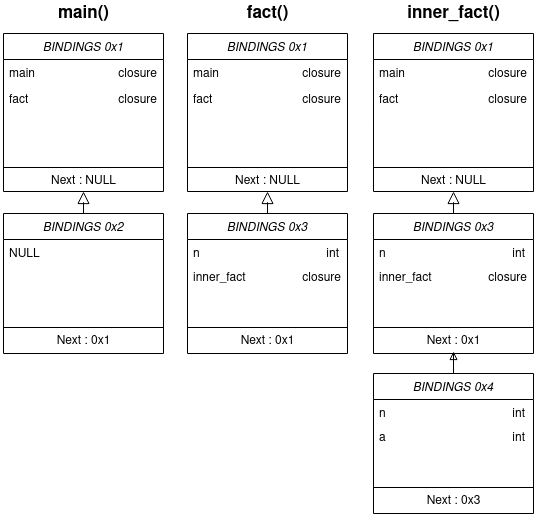
\includegraphics[scale=0.5]{1.png}
     \caption{Frame Diagram - lower is more local to the function}
     \label{framdia}
 \end{figure}
 \begin{figure}[H]
     \begin{verbatim}
        int fact(int n) {
            int inner_fact(int n, int a) {
            if (n==0) return a;
            return inner_fact(n-1,a*n);
            }
            return inner_fact(n,1);
            }
           
            int main() { return fact(10);}
     \end{verbatim}
     \caption{A simple factorial function}
     \label{codefordia}
 \end{figure}
 \subsubsection{interpret\_tree} 
 This is the main recursive function of the interpreter, which is called with the entry point 'main', and is where most of the processing happens.
 The entire function is effectively a switch statement, with a case for each \textbf{NODE} type:
 \paragraph{LEAF}
 If the node is a leaf, it contains either a constant, string literal, or identifier. For constants and string literals, a new \textbf{VALUE} struct is constructed with the value required. If it is an identifier, it will lookup the name in the list of frames described in section \ref{env}, and if it exists return it, otherwise through an 'undefined variable' error (since all variable declarations come at the top of a block).
 \paragraph{TILDE ($\sim$)} A tilde indicates a declaration. We call the \textbf{interpret\_tilde} function (simply refactored out of \textbf{interpret\_tree} for code readability), which checks if the declaration is of a simple type (integer, string literal), and creates an empty binding (initialized to 0 for integers) if the declaration is of type \textbf{int x;}, else performs the assignment if the declaration is of type \textbf{int x = 1} (or any other assignment operation). If it is not a simple type (i.e. a declaration of an inner function), then we simply call \textbf{interpret\_tree} again.
 \paragraph{D} A 'D' indicates a function definition. For this we simply declare a new closure within the current scope. 
 \paragraph{;} A semicolon indicates a sequence of statements, so we simply recurse on the left and then the right. However we encounter an interesting problem here; that of the early return statement. Take the following code sample:
 \begin{figure}[H]
    \centering
    \begin{subfigure}{.5\textwidth}
      \centering
      \begin{verbatim}
        int main() {
            if (1==1) {
                return 1;
            } 
            return 0;
        }
      \end{verbatim}
      \caption{Code Snippet}
      \label{code}
    \end{subfigure}%
    \begin{subfigure}{.5\textwidth}
      \centering
      \begin{verbatim}
        D
        d
          int
          F
            main
        ;
          if
            ==
              1
              1
            return
              1
          return
            0
      \end{verbatim}
      \caption{Corresponding AST}
      \label{ast}
    \end{subfigure}
    \caption{The Return problem}
    \label{rp}
    \end{figure}
Looking at Figure \ref{code}, it is clear that the function should return 1; however, looking at the AST, if we process a sequence of statements in the correct order, how are we to know that we should not process the next statement in the sequence, in the case of an early return? \\\newline
Fortunately, the solution is quite simple. We simply have a pair of global variables: one to indicate that we are processing a sequence, and one to indicate that we have returned. So, once we reach a ';' node, we mark that we are processing a sequence. Then we process the left node. If we reach a return statement, we set our return flag. Once we come back up the tree to the initial ';' node, we check to see if we have returned early. If we have, we just return the result on the left, and do not process the right.
\paragraph{Assignment (=)} On this node, we know we are below the declaration block as \textbf{parse\_tilde} handles this. We recurse on the left, to hit the \textbf{LEAF} case described above (to check if the variable is declared), and then cast the name on the left to a \textbf{TOKEN}, and then simply perform the assignment of whatever is on the right to the name in the current scope. 
\paragraph{Arithmetic (+,-,*,/,\%) and Boolean (<,>,<=,>=,==,!=)} We know that whatever is on the left and right of this node must resolve to an integer, so we simply recurse on both sides, then return a new value with the arithmetic operation performed on the results of the recursion. The same is done for boolean operations, but we simply return a boolean \textbf{VALUE}.
\paragraph{RETURN} Returns the result of recursing on the left child.
\paragraph{APPLY} We first resolve the parameters of the call to a \textbf{VALUELIST} (a linked list of values), and pass the current frame, the resolved parameters, and the name of the function to \textbf{call}, which does as is described in section \ref{flow}.
\paragraph{IF} We call the \textbf{parse\_if} method, which first declares a new scope for the block. Then we evaluate the condition of the branch by calling \textbf{interpret\_tree}. Depending on the result, we interpret either the consequent (IF block) or the alternative(ELSE block), if there is one (and with its own scope).
\\\newline There are additional helper functions in the \textbf{interpreter.c} file but what has been descibed covers the main functionality of the interpreter. The final result of interpretation is whatever is contained in the return statement in 'main'.
\subsection{Intermediate Representation}\label{inmed}
TAC is generated in a similar way to the interpreter, with a walk over the AST generated by the parser using a similar recursive function. The TAC aspect of the compiler is most likely the weakest aspect of my implementation, as it has a few problems that were not addressed in the most correct way possible due to time constraints. These will be discussed in the limitations section.
\subsubsection{Environment}
Scope is handled in a similar way to the interpreter, with an analogue of the interpreter \textbf{FRAME}. This FRAME is the same as is used in the MCG section and will be described in the corresponding section of the report. 
TAC has the addition of an \textbf{ENV} struct, which manages the allocation of labels. In retrospect this was overengineered and could've simply been handled with an integer counter.
The \textbf{ENV} struct simply holds a counter, which is incremented every time a label is generated. 
\subsubsection{TAC Instructions}
The TAC struct has 3 members; an integer 'op', to indicate the type of operation, a \textbf{TAC*} next, which indicates the next operation in the sequence, and a union whose member can be any of a
 STAC, PROC, LOAD, LABEL, IFTEST, GOTO, CALL or RTN. 
\paragraph{STAC} This struct is the basic type of TAC (Simple TAC - STAC), which is used for arithmetic operations. It takes 3 \textbf{TOKEN}s; two sources and a destination.
\paragraph{PROC} This struct is for TAC instructions that indicate the start of a procedure. It takes a \textbf{TOKEN} 'name' and the arity of the procedure. 
\paragraph{LOAD} A load instruction. It takes a source and a destination. It is also used for \textbf{STORE} operations, as they take the same number of parameters.
\paragraph{LABEL}A label for control transfers within a procedure. It takes a label name.
\paragraph{IFTEST} An 'if' condition, indicating a conditional branch. It takes two operands to make a comparison between, an integer 'op' indicating the kind of comparison to make (these integers are the same as defined in \textbf{C.tab.h} for '$<$' '$>$', 'LE\_OP', 'GE\_OP' 'NE\_OP' and 'EQ\_OP'), and a label to jump to if the condition evaluates to false. 
\paragraph{GOTO} An unconditional branch, taking a label to jump to.
\paragraph{CALL} Indicating a call to a function. It takes a \textbf{TOKEN} 'name' (the name of the function), the arity and a \textbf{TOKENLIST} 'args', which are the arguments to the function. These may be any of a constant, another function, a temporary (in the case of some operation e.g. '1+1' being passed as a parameter, eagerly evaluated and assigned to a temporary), or a variable name.
\paragraph{RTN} Indicating a return from a function. It contains a union of \textbf{CALL} (in the case of a function being returned) or a \textbf{TOKEN} in the case of a variable or constant, or temporary (again, in the case of an operation, eagerly evaluated and assigned to a temporary).
\\\newline There is also \textbf{ENDPROC}, which indicates the end of a procedure and takes no parameters. These are all the forms of operation that a TAC can take. These choices will be justified and evaluated in the limitations section. 
\subsubsection{Control Flow}
  The AST enters the \textbf{gen\_tac} function, which initializes the environment and passes the tree to the main recursive function \textbf{gen\_tac0}, which walks the tree. It then takes the generated TAC and performs another pass on it to generate the graph of basic blocks, although this was later taken out as it was not utilized, which is justified later on. 
\subsubsection{gen\_tac0}
\textbf{gen\_tac0} takes as input an AST, and returns a sequence of TAC instructions. 
\paragraph{LEAF} We simply \textbf{LOAD} whatever is in the leaf into a new temporary.
\paragraph{TILDE ($\sim$)} We call \textbf{parse\_tilde}, which checks if the declaration is of type '\textbf{int x;}', '\textbf{int x = 1}' or a function declaration. If it is the first, then we perform a \textbf{LOAD} as in the case of a LEAF, and subsequently a \textbf{STORE}. We also assign the temporary to the variable in the FRAME, so that we know that temporary contains that variable. If it is the second, 
We call \textbf{gen\_tac0} on the right to load the result of the assignment into a temporary (if the assignment is of type \textbf{int x = 1} then the resulting TAC would be a \textbf{LOAD} instruction for 1, if the assignment is of type \textbf{int x = 1+1} the TAC would be a \textbf{STAC}, and then we assign whatever the destination temporary is to the variable in the FRAME and generate the corresponding \textbf{STORE} instruction. If it is a function declaration, we simply call \textbf{gen\_tac0} again.
\paragraph{D} We call \textbf{gen\_tac0} on the left and right, and append an \textbf{ENDPROC}. 
\paragraph{d} Indicates a function definition on the right and return type on the left. We recurse on the right.
\paragraph{F} Indicates a function definition. We create a new \textbf{PROC} instruction.
\paragraph{;} A sequence; we recurse on the left and right. Since we are not directly computing an answer as in the interpreter, the early return problem is not relevant here. 
\paragraph{Assignment (=)} Similar to the procedure in \textbf{parse\_tilde} we recurse on the right, and store whatever is the final destination of the TAC returned in the \textbf{TOKEN} on the left.
\paragraph{Arithmetic (+,-,*,/,\%) and Boolean (<,>,<=,>=,==,!=)} For arithmetic, we recurse on the left and get the final destination of the TAC returned, then recurse on the right and do the same. We then create a new \textbf{STAC} with the operands as these two destinations and the destination address as a new temporary. Booleans do not need to be handled in this main recursive function as we are not computing as in the interpreter, so they are handled by the \textbf{parse\_if} function which is described later. 
\paragraph{RETURN} We call \textbf{new\_return}, which has three cases for each possible return type. If the type is a LEAF (i.e. constant, variable or closure), we create a new \textbf{RTN} with the corresponding \textbf{TOKEN}. If the type is an operation (e.g. 'return 1+1'), we call \textbf{gen\_tac0}, and create a new \textbf{RTN} with whatever the final destination of the generated TAC is. If the type is APPLY, we create a new \textbf{CALL}, with the same procedure as is described in the APPLY section below. 
\paragraph{APPLY} We call \textbf{new\_call}, which generates a \textbf{CALL} and adds the name, arity and argument \textbf{TOKEN}s. 
\paragraph{IF} We call \textbf{parse\_if}, which creates a new \textbf{IFTEST} with the opcode and two operands in the condition. If the block is of type 'IF\dots ELSE', We generate the code for the consequent and alternative with a resursive call on \textbf{gen\_tac0}, and create a \textbf{GOTO} instruction for the end of the consequent which points to the next block below the alternative, and a \textbf{LABEL} for the alternative which the \textbf{IFTEST} points to. If the block is only an IF and no ELSE, we generate the code for the consequent again with a resursive call on \textbf{gen\_tac0}, and generate a new label below the consequent which the \textbf{IFTEST} points to. 
\\\newline This covers all the nodes in the parse tree the TAC generator is able to parse. 
\subsubsection{Basic Block Generation}
A basic block is a straight line code sequence that contains no control transfers\supercite{cooper2011engineering}. In the case of generating basic blocks from TAC sequences, a basic block: 
\begin{itemize}
  \item Begins with a leader
  \item Continues until reaching another leader
  \item Ends with the instruction preceeding a leader
\end{itemize}
A leader can be: 
\begin{itemize}
  \item The first instruction in a program 
  \item The target of a jump
  \item The instruction immediately following a jump 
\end{itemize}
Leaders can also be instructions that follow an instruction that can throw an exception and exception handlers\supercite{aho1986compilers}, however this is not relevant for --C.
The basic blocks are generated with a pass over the generated TAC from \textbf{gen\_tac0}. Unfortunately they were never put into use as due to time constraints, I could not do any machine-independent optimization. 
\subsubsection{Control Flow Graph (CFG)}
The graph of basic blocks forms a Control Flow Graph\supercite{cfg}, which represents all the paths of execution through a program. It is the basic structure for optimization. A basic block node in a CFG can technically have unlimited edges (for example in the case of a switch statement),
but in the case of --C where the only control transfers we deal with are if\dots else blocks and function calls, the maximum number of edges is two. 
\begin{figure}[H]
  \begin{verbatim}
    typedef struct bb {
    TOKEN* id; 
    TAC* leader;
    struct bb *nexts[2];
    }BB;
  \end{verbatim}
  \caption{Basic Block struct}
  \label{bb}
\end{figure}
Figure \ref{bb} shows the structure of a basic block. It contains the id of the block, the straight line sequence starting at 'leader', and the array of next blocks, which may be any number from 0 to 2.
\paragraph{gen\_bbs} gen\_bbs() takes as input a sequence of TAC and outputs a graph of basic blocks, represented as an adjacency list. We start at the first instruction in the TAC sequence and label this as the first block leader. we step through the sequence until reaching a \textbf{IFTEST}, \textbf{GOTO}, \textbf{LABEL} or the end of the sequence.
Once we reach the end of a basic block, we label the block with an id of either the label name if the leader is a label, or an integer otherwise (which is incremented with every new block). \\\newline Then we fill in the 'nexts' array. If we have already parsed the basic block to which the current block transfers control to, we fill in its position in the 'nexts' array with a pointer to this block. If we haven't parsed it, we fill it in with a NULL pointer, and update it once this block has been parsed. We do this for every edge of a block. The result looks like this: 
\begin{figure}[H]
  \centering
  \begin{subfigure}{.5\textwidth}
    \centering
    \begin{verbatim}
      int main() {
        int x = 1;
        if(x==1){
          return 0;
        } 
        else{
          return 1;
        }
      }
    \end{verbatim}
    \caption{Code Snippet}
    \label{code2}
  \end{subfigure}%
  \begin{subfigure}{.5\textwidth}
    \centering
    \begin{verbatim}
      BLOCK #0
      PROC main 0
      LOAD 1 t0
      STORE t0 x
      IF (x==1) L1
      LINKS TO : 1 L1
      
      BLOCK #1
      RETURN 0
      GOTO L2
      LINKS TO : L2
      
      BLOCK #L1
      LABEL L1
      RETURN 1
      LINKS TO : L2
      
      BLOCK #L2
      LABEL L2
      ENDPROC
    \end{verbatim}
    \caption{Basic Blocks generated}
    \label{bbgen}
  \end{subfigure}
  \caption{Basic Block Generation}
  \label{bbdemo}
  \end{figure}
\subsection{Intermediate Code - Limitations}
There are some considerable limitations in the TAC generation stage, which lead to consequences in the MCG. You will have noticed I make no mention of closures; this is because in my TAC stage I make no effort to generate closures. As a result, I am having to create these in the MCG stage whilst parsing the TAC. Another consequence of this is the inability to 'flatten' the structure of TAC; inner functions cannot be separated out from regular functions because there is no mechanism to do so without closures. As a result, I had to implement a less than ideal workaround. There is a depth counter which increments every time we recurse on a function, so that the depth at any function lexically defined in the global scope is at depth 0 and an inner function would be at depth 1 and so on. Then any function defined at a depth of 1 or more has the TAC code \textbf{INNER\_PROC}, so that the MCG parser can recognize this as a function and build a closure.
Had I properly implemented the TAC stage, MCG would have been much simpler and effectively template-based, whereas now I am having to 'pick up the pieces' in MCG and build a new environment as I parse the TAC. 
\\\newline Furthermore, my TAC most likely could have been higher-level; instructions such as \textbf{STORE} and \textbf{LOAD} make it dangerously close to assembly, and reduce the portability and legibility of the TAC; a higher-level TAC design would better hide implementation details, and a smaller instruction set (the current system has 15 TAC instructions) would make translation to MCG simpler.
\\\newline Details in regard to possible optimizations will be discussed in the Further Improvements section.
\subsection{MIPS Assembly Generation}
MIPS is generated with a recursive function acting on the TAC sequence generated as per section \ref{inmed} (basic blocks are not passed in since no optimization was done).
\subsubsection{Architecture}
MIPS is a RISC instruction set architecture created in the 1980s\supercite{price1995mips} designed for the R2000 microprocessor. It has 32 (32-bit) general purpose registers and a few special registers:
\begin{figure}[H]
  \begin{tabular}{c|l}
    \$zero & The value 0 \\\hline
    \$v0-v1 & expression evaluation and function results \\\hline
    \$a0-a3 & first four parameters for subroutine \\\hline 
    \$t0-t9 & temporary variables \\\hline 
    \$s0-s7 & saved values representing final computed results \\\hline 
    \$ra & return address
  \end{tabular}
  \caption{MIPS registers}
  \label{reg}
\end{figure}
Figure \ref{reg} illustrates the register usage in MIPS architecture. In this implementation, \$v0 is always used for syscalls and \$v1 is used for function returns. The $s$ registers are not used, as they are not required in my implementation, however I will talk about how they could be used to speed up execution later on in this section.
\subsubsection{Environment}
An activation record (or frame as it is sometimes referred to) is simply a collection of information that can be useful for the calling and returning from procedures. It can contain\supercite{compilers}: 
\begin{itemize}
  \item Parameters
  \item Returned values
  \item Control link (or static link)
  \item Access link; a pointer to data the procedure used that is located in another frame
  \item Saved machine status
  \item Local data
  \item Temporaries 
\end{itemize}
I will not go into detail on all of these as they are not all relevant to my implementation, but a few of these items are stored in the current activation record: 
\paragraph{Local Data} The contents of all registers in use by a procedure are saved into the activation record. 
\paragraph{Static Link} The static link of the current frame; that is, the depth in the lexical scope (although as it turns out, due to my choice of implementation this is not used).
In addition to these, the activation record (AR) also contains the arity of locals. \\\newline
This is the contents of the AR as is generated in the machine code, however due to a change of strategy, a lot of this information is now redundant. 
The machine code generator uses the same \textbf{FRME} (an analogue of the interpreters \textbf{FRAME}) as the TAC environment, and it is used to track where variables are (i.e. in register or in memory):
\begin{figure}[H]
  \begin{verbatim}
typedef struct clsure {
  FRME* env;
  TAC* code;
  int processed;
} CLSURE;

typedef struct bnding {
  TOKEN* name;
  int type;
  union {TOKEN* loc; CLSURE* clos;};
  struct bnding* next;
} BNDING;

typedef struct frme {
  BNDING* bindings;
  int size;
  int stack_pos;
  struct frme* next;
}FRME;
  \end{verbatim}
  \caption{MCG FRME}
  \label{frme}
\end{figure} 
The \textbf{FRME} contains a size (this is the same as the size of the AR, it's just included here for convenience), the stack position (which we will come to later) and the next frame. The binding (\textbf{BNDING}) is almost identical to the binding in the interpreter, except that in place of a \textbf{VALUE} struct it is simply a union of either closure or location (register).
A closure (\textbf{CLSURE}) is again almost identical to a closure in the interpreter, with the addition of a 'processed' flag, which is a workaround due to the lack of closures generated in TAC, which will be explained later in this section. 
\\\newline Instead of the recommended heap allocation for storing ARs, I opted for heap allocation. This was for multiple reasons; on the suggestion of a peer that the stack would be faster - in general it is, as stack pointer relative locations can be determined at compile time causing runtime access speeds to be very fast, versus heap allocation which has to be done during run time via \textbf{sbrk}, and the other reason being for me at least the stack was simpler to understand rather than having to keep track of pointers in the heap. However, I believe now that I overestimated the speed savings as access speeds are fairly insignificant.
\subsubsection{Control Transfer}
Although basic blocks are not passed to the MCG for reasons previously mentioned, a basic block is a useful term to describe when we transfer control. In this section assume that when we say 'frame' we are referring to an activation record. We know that four basic things must happen when a transfer of control within execution occurs:
\begin{itemize}
  \item Frame creation 
  \item Frame deletion
  \item Frame saving
  \item Frame restoration
\end{itemize} 
These four actions occur when we enter a basic block, exit a function, exit a basic block, and return to a function after some control transfer respectively.
\paragraph{Frame Creation} At the start of a basic block, we must calculate the size of the frame we need to create. This is done by counting the number of locals, and adding to this a fixed number that is the basic information any frame must contain, and finally adding the arity in the case of a procedure. A typical frame would look something like this: 
\begin{figure}[H]
  \begin{verbatim}
    # Creating new frame
    addiu $sp, $sp -12
    li $t1, 12
    sw $t1, 0($sp)
    li $t2, 1
    sw $t2, 4($sp)
    li $t3, 0
    sw $t3, 8($sp)
    # End of creating frame
  \end{verbatim}
  \caption{Typical MC for a frame}
  \label{mcgenframe}
\end{figure}
In Figure \ref{mcgenframe} we can see that we first decrement the stack pointer by the size of the frame, store the size of the frame in the first location, the static link in the second and finally the arity plus the number of locals. Space is allocated for these in case the frame needs to be saved but they are not actually stored on the stack until necessary.

\paragraph{Frame Deletion} When we exit a function, we no longer require this frame, and so to save stack space we simply increment the stack pointer by the size of the frame to point to the next available location.
\paragraph{Frame Saving} When we transfer control from within a function, we must save the contents of the registers as they are not guaranteed to be unchanged by whatever function we call. We must save all variables local to a function before we transfer control. Saving a frame will typically look like this: 
\begin{figure}[H]
  \centering
  \begin{subfigure}{.5\textwidth}
    \centering
    \begin{verbatim}
      int f() {
         return 1;
      }
      int main() {
        int x = 3;
        f();
        return x;
      }
    \end{verbatim}
    \caption{Code Snippet}
    \label{code3}
  \end{subfigure}%
  \begin{subfigure}{.5\textwidth}
    \centering
    \begin{verbatim}
      main:
      # Creating new frame
      addiu $sp, $sp -16
      li $t1, 16
      sw $t1, 0($sp)
      li $t2, 1
      sw $t2, 8($sp)
      li $t3, 1
      sw $t3, 4($sp)
      # End of creating frame
      
      li $t0,3
      
      # Saving frame
      sw $t0 12($sp)
      # End of saving frame
      
      jal f
    \end{verbatim}
    \caption{MCG generated - segment}
    \label{savfram}
  \end{subfigure}
  \caption{Saving a frame}
  \label{frmsaving}
  \end{figure}
Figure \ref{frmsaving} shows the saving of the frame of 'main' before transferring control. we store the local 'x' in its position on the stack before jumping to 'f()'.
\paragraph{Frame Restoration} After we return from a jump in a function, we must restore the state of the registers prior to the jump. Using the same example as above: 
\begin{figure}[H]
  \begin{verbatim}
    main:
    # Creating new frame
    addiu $sp, $sp -16
    li $t1, 16
    sw $t1, 0($sp)
    li $t2, 1
    sw $t2, 8($sp)
    li $t3, 1
    sw $t3, 4($sp)
    # End of creating frame

    li $t0,3

    # Saving frame
    sw $t0 12($sp)
    # End of saving frame

    jal f
    # Restoring frame
    lw $t0  12($sp)
    # End of restoring frame
    lw $v1 t0
    addiu $sp, $sp 16
    jr $ra
  \end{verbatim}
  \caption{Restoring a frame}
  \label{rstfrme}
\end{figure}
Figure \ref{rstfrme} Shows the restoration of the current frame after a jump. We load the local 'x' from its position on the stack back to the register it was previously in after returning from 'f()'. \\\newline
These are the main operations for maintaining proper state through control transfer in a program.
\subsubsection{Control flow}
The control flow for the MCG is similar to the interpreter. We enter via \textbf{gen\_mc} which generates some initial instructions that go at the top of every program (.global premain, .text etc). Then we enter \textbf{gen\_globframe} which generates the global frame; it simply steps through the TAC, and adds any variable delcarations to the global \textbf{FRME}, and generates closures for any procedures. The global frame (AR) creation is done in a function 'premain', which does the global initialization and then jumps to main. In \textbf{gen\_mc}, we step through the global \textbf{FRME} until we find 'main', and then we call the main recursive function \textbf{gen\_mc0}.  \textbf{gen\_mc0} is again a large switch statement with a case for each TAC instruction type: 
\subsubsection{gen\_mc0}
\textbf{gen\_mc0} takes as input a sequence of TAC instructions and outputs a sequence of MIPS assembly instructions, mainly via template-based generation on the fly. 

\end{document}